\graphicspath{ {./content/exp/figure/} }

\section{Experiments and results}\label{sec:4}


For this experiment the goal is to find the best position for one cameras network. To have better result of the 1st experiment (less camera and better coverage, see figure 3 and 5) it is necessary to add one more degrees of freedom. The Pan was chosen because is a more realistic solution and interesting for snap workable image to use for video surveillance (with the adequate pan you can do face recognition \cite{an2012face} or object detection)\cite{parupati2011collaborative} .
 For the experiment the camera accepts a pan angle $\theta$ between $-\pi/4$  to  $\pi/4$ 

\begin{figure}
  \centering
  \hspace*{\fill}
  %\subfigure[]{\label{subfig:4a}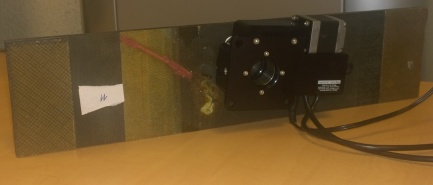
\includegraphics[width=0.3\linewidth]{fig4a.png}} \hfill
  %\subfigure[]{\label{subfig:4b}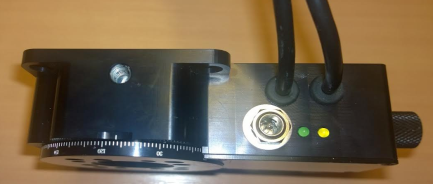
\includegraphics[width=0.3\linewidth]{fig4b.png}} 
  %\hspace*{\fill} \\ \hspace*{\fill}
  %\subfigure[]{\label{subfig:4c}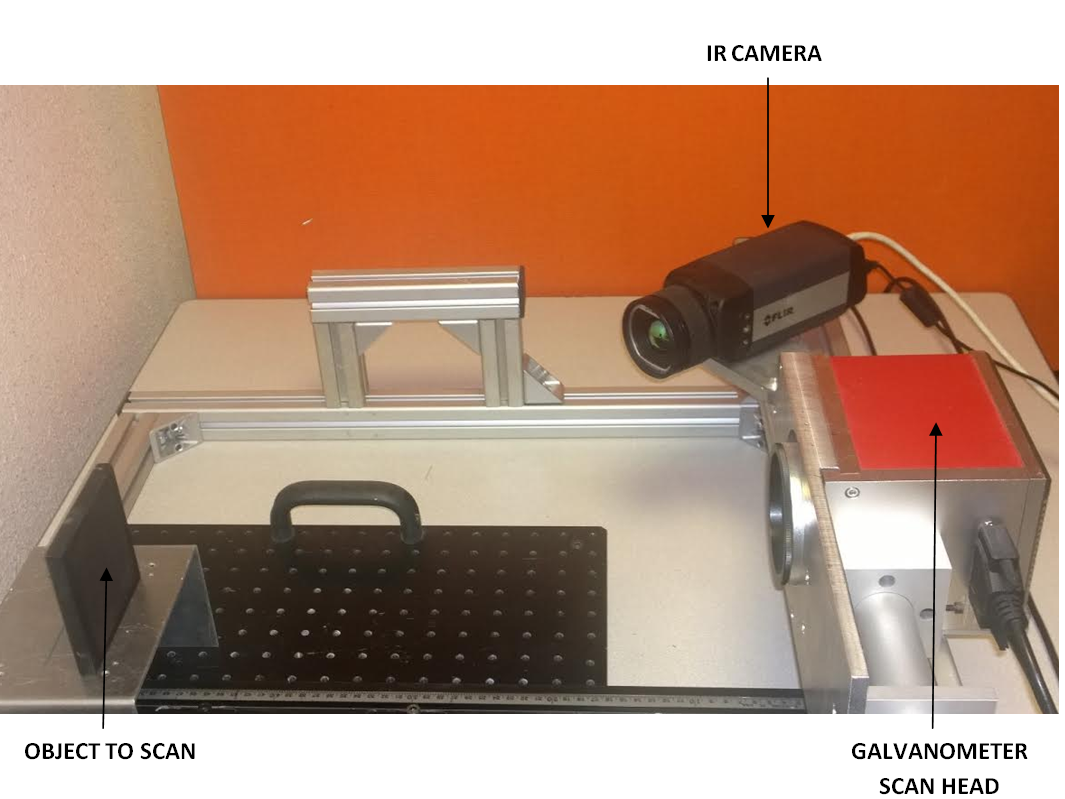
\includegraphics[width=0.3\linewidth]{fig4c.png}}
	{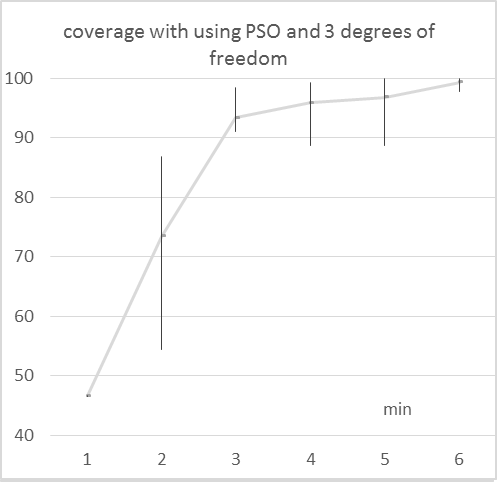
\includegraphics[width=0.7\linewidth]{fig7.png}}
  \hspace*{\fill}
  \caption{%(a)-(b) Device for positioning the composite material - 
	Percentage of coverage with n number of camera (1 to 6). The camera was positioning with PSO algorithm to optimize the position on X, Y and the pan of pose.}
  \label{fig:4}
\end{figure}
\begin{figure}
  \centering
  \hspace*{\fill}
  %\subfigure[]{\label{subfig:4a}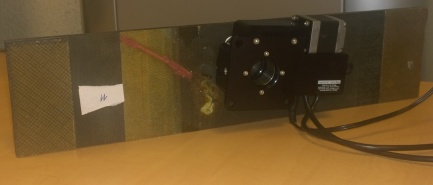
\includegraphics[width=0.3\linewidth]{fig4a.png}} \hfill
  %\subfigure[]{\label{subfig:4b}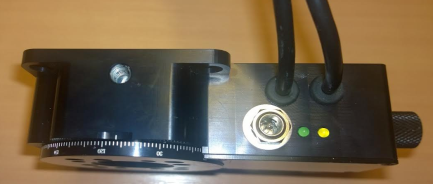
\includegraphics[width=0.3\linewidth]{fig4b.png}} 
  %\hspace*{\fill} \\ \hspace*{\fill}
  %\subfigure[]{\label{subfig:4c}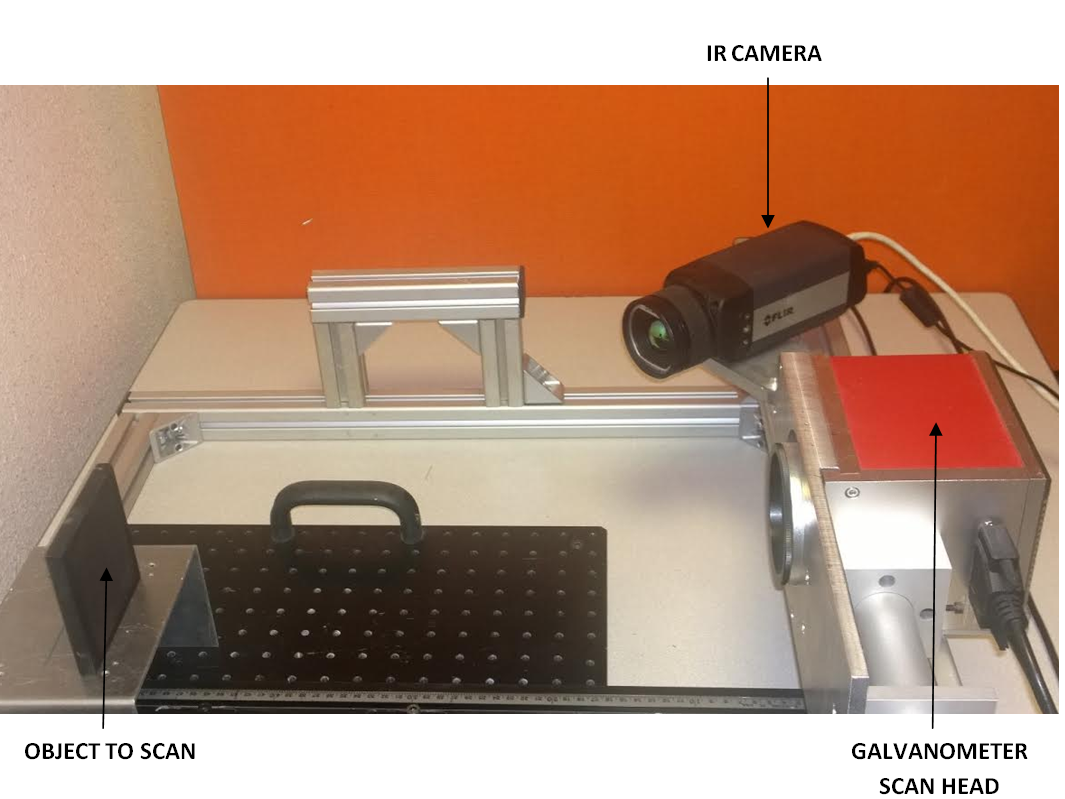
\includegraphics[width=0.3\linewidth]{fig4c.png}}
	{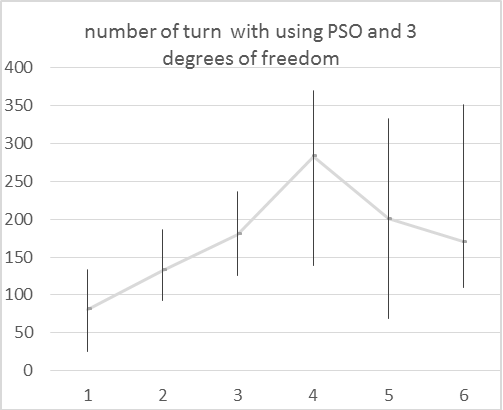
\includegraphics[width=0.7\linewidth]{fig8.png}}
  \hspace*{\fill}
  \caption{%(a)-(b) Device for positioning the composite material - 
	Number of iterations before converged solution.  The algorithm implement for the PSO stop when it’s impossible to find best solution after 100 random set of camera pose}
  \label{fig:4}
\end{figure} 
After this last experimentation, it’s interesting to compare the result for the speed and the quality of coverage.
	Add one more degrees of freedom in the system can help for have better solution of coverage, because when with 2 degrees of freedom PSO need 21 cameras for a complete coverage (figure 5) the same experience, but with 3 degrees of freedom (x y and Ɵ) find an solution with 6 cameras (figure 7).
But even if the time computation is better compared to PSO with 2 degrees of freedom, it’s still little slower than random walk with 2 degrees of freedom  (compare figure 8 and  figure 4) 



\subsection{Visualization with simulation robot tool }\label{subsec:42}


To the visualization of the result, the tool is used from the robotic V-rep \cite{verp} this tool can help to visualize the limit of PSO on the real world.

After some experimentation is interesting to use the result find with Matlab, the solver model and the PSO (for 3 degrees of freedom) with a simulation system for robots. This experiment with robot simulation (see figure 9) can proof at the same time the efficiency of the algorithm and can help to visualize the limit of the system

\begin{figure}
  \centering
  \hspace*{\fill}
  %\subfigure[]{\label{subfig:4a}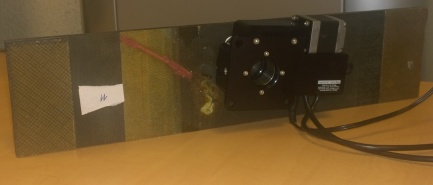
\includegraphics[width=0.3\linewidth]{fig4a.png}} \hfill
  %\subfigure[]{\label{subfig:4b}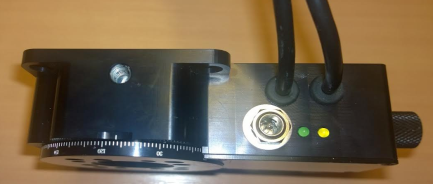
\includegraphics[width=0.3\linewidth]{fig4b.png}} 
  %\hspace*{\fill} \\ \hspace*{\fill}
  %\subfigure[]{\label{subfig:4c}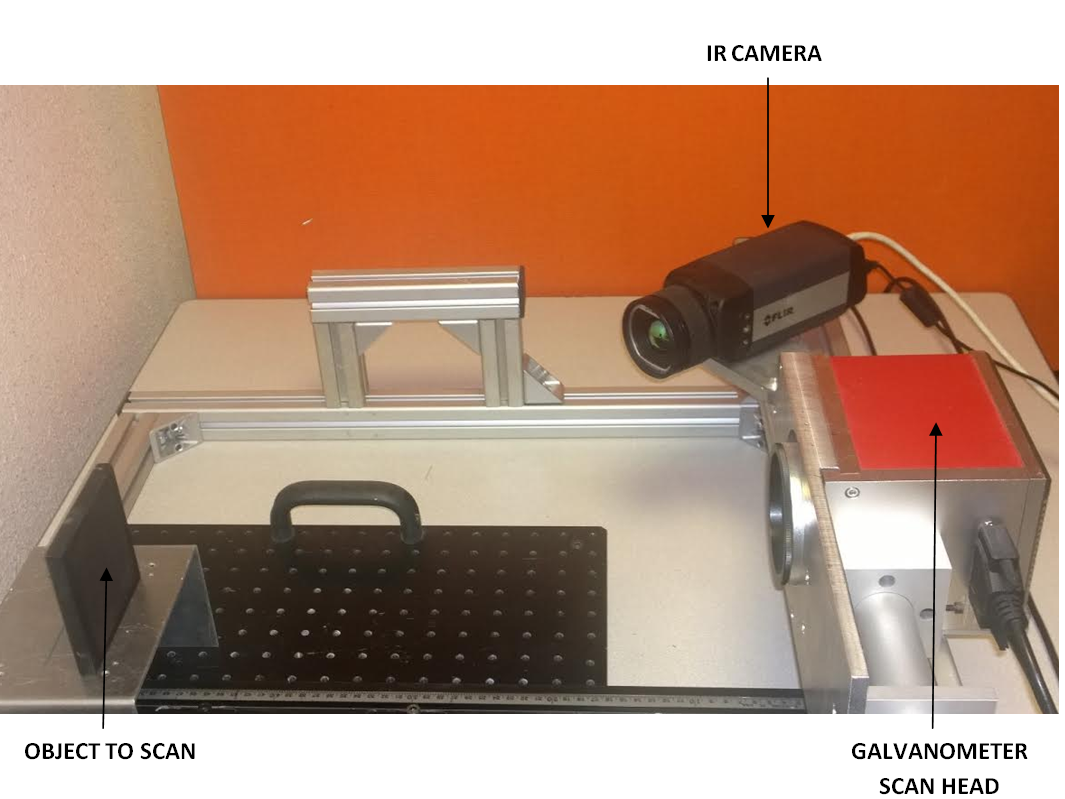
\includegraphics[width=0.3\linewidth]{fig4c.png}}
	{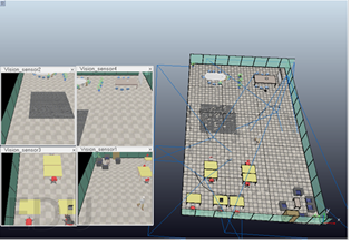
\includegraphics[width=0.7\linewidth]{fig9.png}}
  \hspace*{\fill}
  \caption{%(a)-(b) Device for positioning the composite material - 
	The result of one experimentation with four camera. The position of the camera and the pan is implement in a robot simulator for have a visualization of the final result}
  \label{fig:4}
\end{figure} 

%%% Local Variables: 
%%% mode: latex
%%% TeX-master: "../../master"
%%% End: 
